\documentclass[aspectratio=169,11pt]{beamer}
\usepackage[utf8]{inputenc}
\usepackage[T1]{fontenc}
\usepackage[english]{babel}
\usepackage{amsmath,amssymb,booktabs}
\usetheme{default}
\usecolortheme{seahorse}
\setbeamertemplate{navigation symbols}{}
\setbeamertemplate{footline}[frame number]
\newcommand{\A}{\mathrm{A}}
\newcommand{\N}{\mathrm{N}}

\title{Artificial Intelligence in the Knowledge Economy}
\subtitle{Ide \& Talam\`as (2025), Repository 5}
\author{William Gradost}
\date{September 17, 2026}

\begin{document}

\begin{frame}[plain]\titlepage\begin{center}\small
\url{github.com/wbgradost/ai-05-ide}
\end{center}\end{frame}

\begin{frame}{1. The question and the mechanism}
\textbf{Question.} Who gains when AI agents enter a knowledge hierarchy, and
does the answer depend on capability, autonomy, or both?

\medskip
Production problems have unknown difficulty $x\sim U[0,1]$. A human with
knowledge $z$ solves a fraction $z$ alone. Workers handle routine problems;
solvers handle exceptions that workers cannot solve.

\medskip
\begin{block}{Core mechanism}
AI changes both the set of tasks that can be performed and the set of roles in
which compute can be used. This changes matches, occupational composition, and
the division of surplus.
\end{block}
\end{frame}

\begin{frame}{2. The pre-AI economy}
There is a unit mass of humans, one unit of time, and knowledge $z\in[0,1]$.

\begin{itemize}
\item A single-layer producer works alone and expected output is $z$.
\item A two-layer firm has workers of knowledge $z$ and a solver of knowledge
      $s\ge z$.
\item Each request for help costs the solver $h\in(0,1)$ units of time.
\end{itemize}

\[
n(z)h(1-z)=1,\qquad n(z)=\frac{1}{h(1-z)}.
\]

Under the maintained case $h<h_0$, Proposition 1 gives the efficient,
positively assortative hierarchy $W\preceq S$ with no independent human
producers.
\end{frame}

\begin{frame}{3. Capability and autonomy are different}
An AI agent has fixed capability $z_{AI}<1$ and uses one unit of compute.

\begin{center}
\begin{tabular}{lll}
\toprule
 & Autonomous AI & Non-autonomous AI\\
\midrule
Independent production & yes & no\\
Worker/co-worker role & yes & no\\
Solver/co-pilot role & yes & yes\\
Compute price (abundant case) & $r=z_{AI}$ & $r=0$\\
\bottomrule
\end{tabular}
\end{center}

\medskip
Capability says how difficult a problem the agent can solve. Autonomy says
whether it can pursue production without a human.
\end{frame}

\begin{frame}{4. Autonomous equilibrium and occupational displacement}
Autonomous AI is always used for independent production. It is also used as a
worker when $z_{AI}\in\operatorname{int}(W)$ and as a solver when
$z_{AI}\in\operatorname{int}(S)$ (Proposition 2, pp.~18--20).

\medskip
\begin{itemize}
\item Basic AI: $z_{AI}\in\operatorname{int}(W)$ displaces humans from routine
      work toward specialized problem solving.
\item Advanced AI: $z_{AI}\in\operatorname{int}(S)$ displaces humans in the
      opposite direction, toward routine work (Proposition 3, p.~21).
\end{itemize}

The same capability parameter therefore has different distributional effects
depending on the occupation it enters.
\end{frame}

\begin{frame}{5. Proposition 5: who wins under autonomous AI?}
Let $w$ be pre-AI wages and $w^\A$ autonomous-AI wages. Define
\[
B=\{z\le z_{AI}:w^\A(z)>w(z)\},\qquad
T=\{z\ge z_{AI}:w^\A(z)>w(z)\}.
\]

The appendix single-crossing lemma gives
$B=[0,z_b)$ and $T=(z_t,1]$. The agent exactly at $z_{AI}$ loses because
$w^\A(z_{AI})=z_{AI}<w(z_{AI})$.

\begin{block}{Exact conditions (v11 p.~24; Appendix \S2.5, pp.~18--21)}
Bottom winners exist iff $z_{AI}>\bar z_{AI}$, where
$\bar z_{AI}\in\operatorname{int}(W)$. Top winners exist for every
$z_{AI}\in[0,1)$ under $h<h_0$.
\end{block}
\end{frame}

\begin{frame}{6. Why the bottom threshold is real}
For the least knowledgeable human, AI creates two forces:
\[
\Delta(0)=w^\A(0)-w(0)
  =\underbrace{\text{share effect}}_{+}
   -\underbrace{\text{match effect}}_{-}\quad\text{(basic AI)}.
\]

The proof constructs $\bar z_{AI}$ from the unique root
$\Delta(0;\bar z_{AI})=0$. It shows $\Delta(0;z_{AI})$ is continuous and
strictly increasing up to the worker/solver boundary. Hence
\[
\Delta(0;z_{AI})>0\quad\Longleftrightarrow\quad z_{AI}>\bar z_{AI}.
\]

For advanced AI, both the match and share effects are positive, so the bottom
wins automatically.
\end{frame}

\begin{frame}{7. Why top winners are not capability-free}
At the top, the share effect always dominates the match effect under the
maintained assumptions. The proof uses
\[
w^\A(1)=\frac1h>w(1)
\]
and the same single-crossing result.

This is not an unconditional statement about every model: the paper notes that
top winners can disappear when $h\ge h_0$, and the superintelligent endpoint
$z_{AI}=1$ makes the most knowledgeable human lose.

\medskip
\textbf{Audit point:} autonomy matters for the regime, but capability remains
inside the winner conditions.
\end{frame}

\begin{frame}{8. Proposition 6: non-autonomous AI}
Let $w^\N$ denote non-autonomous-AI wages. AI can only be a solver, so
$r=0$ and unused compute is idle.

\begin{block}{Adoption threshold (v11 p.~27; Appendix \S2.6, pp.~21--27)}
If $z_{AI}\le w(0)$, AI is not used and occupations and wages equal the pre-AI
equilibrium. If $z_{AI}>w(0)$, only the least knowledgeable humans use AI as a
solver, through a unique cutoff allocation.
\end{block}

The threshold is explicitly about capability relative to the pre-AI bottom
wage, not autonomy alone.
\end{frame}

\begin{frame}{9. Proposition 6: distribution and output}
Proposition 6 also establishes:
\begin{enumerate}
\item Autonomous-AI output is strictly higher than non-autonomous-AI output.
      Autonomous compute can produce; non-autonomous compute must leave some
      capacity idle.
\item With adoption, at least one human loses relative to pre-AI.
\item A neighborhood of the bottom does at least as well under non-autonomous
      AI as under pre-AI or autonomous AI (strictly better when adopted).
\item A neighborhood of the top does weakly worse under non-autonomous than
      under autonomous AI; the inequality is strict below the endpoint.
\end{enumerate}
\textbf{Bottom line:} autonomy changes the opportunity-cost channel and output;
capability controls adoption and the location of winners.
\end{frame}

\begin{frame}{10. A two-type calculation to write by hand}
Take two low types $z_L=0$, one high type $z_H=0.8$, and $h=0.5$. Then
$n(0)=2$. Normalize the high type's outside option to $w_H=0.8$.
\[
Y^0=2(0.8)=1.6,\qquad w_L^0=\frac{1.6-0.8}{2}=0.4.
\]
For capability $q\in(0.4,0.8)$ and one compute unit:
\[
Y^\N=0.8+2q,\qquad Y^\A=1.6+q,
\]
because non-autonomous AI supervises the two low workers while autonomous AI
uses compute independently and leaves the human hierarchy intact.
\[
Y^\A-Y^\N=0.8-q>0.
\]
This is a transparent discrete specialization, not the continuum proof.
\end{frame}

\begin{frame}{11. Where I did not believe the AI}
The tempting summary was: “distributional effects depend on autonomy, not
capability.”

\begin{alertblock}{Verdict}
Too strong. Capability determines the autonomous bottom-winner threshold
$z_{AI}>\bar z_{AI}$ and the non-autonomous adoption threshold
$z_{AI}>w(0)$. Autonomy changes which roles compute can perform and whether
compute has a production opportunity cost.
\end{alertblock}

The paper's two-dimensional taxonomy is more informative than the one-line
gloss.
\end{frame}

\begin{frame}{12. The missing manuscript evidence}
\begin{center}
\IfFileExists{hand/derivation.jpg}{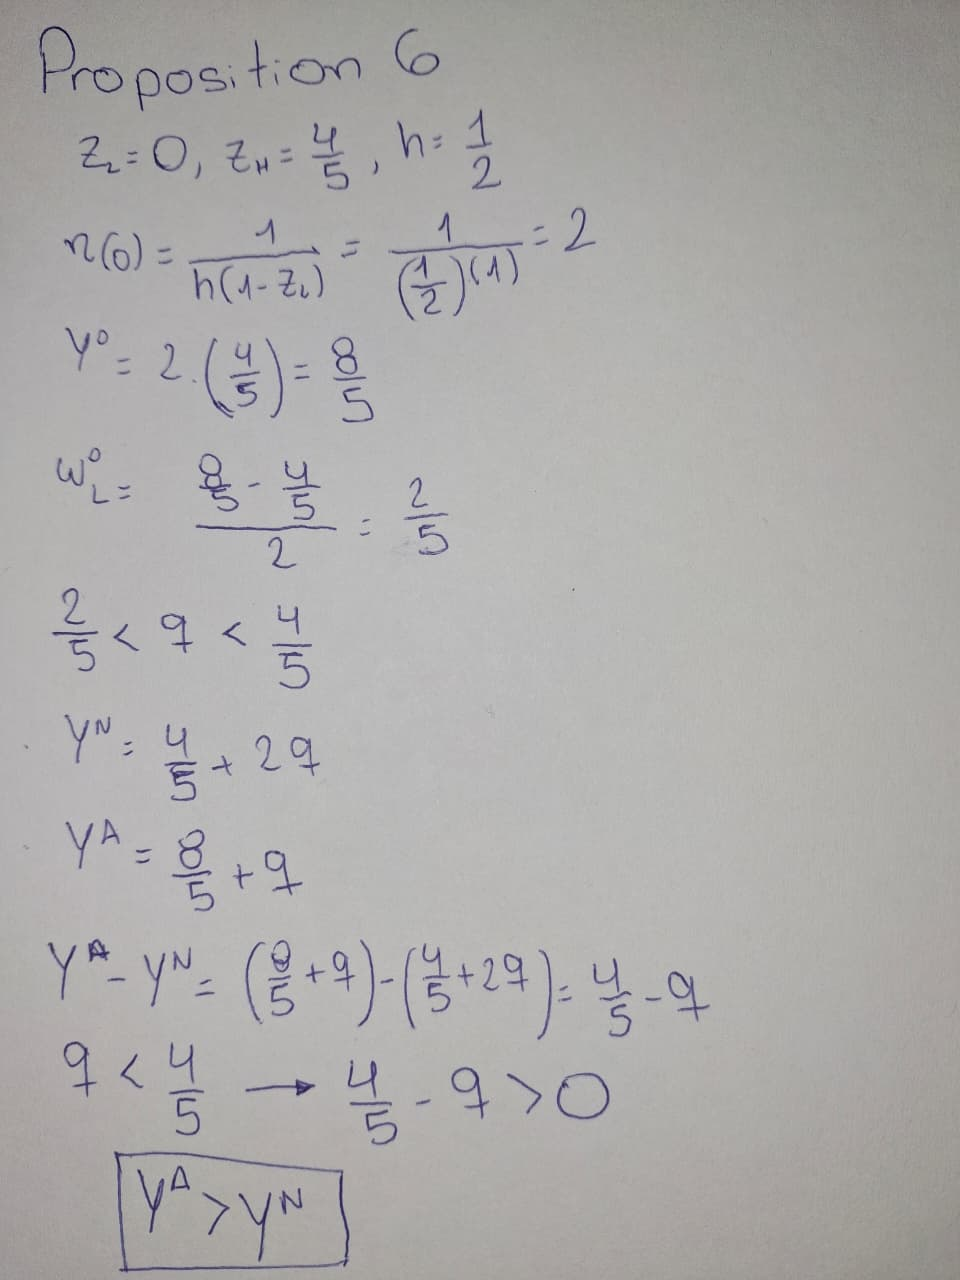
\includegraphics[width=.7\linewidth]{hand/derivation.jpg}}{\fbox{\parbox{.72\linewidth}{\centering\vspace{1em}The author's photograph of the hand derivation will be inserted here.\\[.5em]No synthetic handwriting is used.\vspace{1em}}}}
\end{center}
\end{frame}

\begin{frame}{13. Lean: original claim $\rightarrow$ formal statement}
\textbf{Original paper claim (Proposition 6, item 1):}
\[
Y^{\A}>Y^{\N}\quad\text{when comparing autonomous and non-autonomous AI.}
\]

\textbf{Our Lean target:} a discrete specialization with two low types and one
high type, for $2/5<q<4/5$,
\[
\frac45+2q<\frac85+q.
\]

This is deliberately labelled a specialization: it is not the full continuum
equilibrium statement.
\end{frame}

\begin{frame}{14. Lean proof and interpretation}
\small
The transparent Spec is paired with theorem
\texttt{discreteOutputStrictlyHigher}. It states
\texttt{4/5 + 2*q < 8/5 + q}. The endpoint assumes
\texttt{2/5 < q} and \texttt{q < 4/5}, unfolds the definition, and closes the
inequality with \texttt{linarith}.

\textbf{What Lean verifies:} given the explicit capability interval, the
discrete autonomous-output expression exceeds the non-autonomous expression by
$4/5-q>0$. The paper target compiled and the AppliedModelingLib
\texttt{--fast} check passed.

\medskip
\textbf{What it does not verify:} the paper's wage functions, continuum
matching, Proposition 5's single-crossing threshold, or the full Proposition 6
equilibrium. The result is partial by design.
\end{frame}

\begin{frame}{15. Takeaways}
\begin{itemize}
\item Knowledge hierarchies turn AI adoption into a matching and surplus-sharing
      problem, not just a productivity shock.
\item Autonomous AI always has a productive compute margin; non-autonomous AI
      may be unused and leaves compute idle.
\item Proposition 5: top winners are guaranteed only under the maintained
      assumptions; bottom winners require $z_{AI}>\bar z_{AI}$.
\item Proposition 6: non-autonomous adoption requires $z_{AI}>w(0)$ and shifts
      gains toward the bottom, while autonomous AI generates higher output.
\item Lean checks one honest discrete output mechanism; the manuscript photo is
      the only deliberately pending deliverable.
\end{itemize}
\end{frame}

\end{document}
